\section{Проектирование}
\label{sections:Design}

Этот раздел содержит описание теоретических аспектов работы.
В первую очередь здесь будет детально рассмотрена
структура информационных моделей,
используемых как источник исходных данных для визуализации.
Далее идет описание клиентской и серверной части прототипа,
описание проблем, которых это разделение призвано решить,
а также описание функциональности, которую они будут предоставлять.
Наконец, эта глава также содержит кратких обзор методик,
используемых для повышения производительности визуализации.

\subsection{Описание предметной области}
\label{subsections:DomainModel}

Далее рассматривается структура информационной модели.
В связи с тем, что в качестве целевого формата был выбран  формат Revit,
дальнейшее описание предметной области будет в первую очередь
соответствовать стандартам Autodesk Revit.
Различия с другими форматами, например Industry Foundation Classes (IFC-формат),%
\cite{BuildingSmartIFC}
рассматриваться не будут.

\begin{figure}[ht]
    \centering
    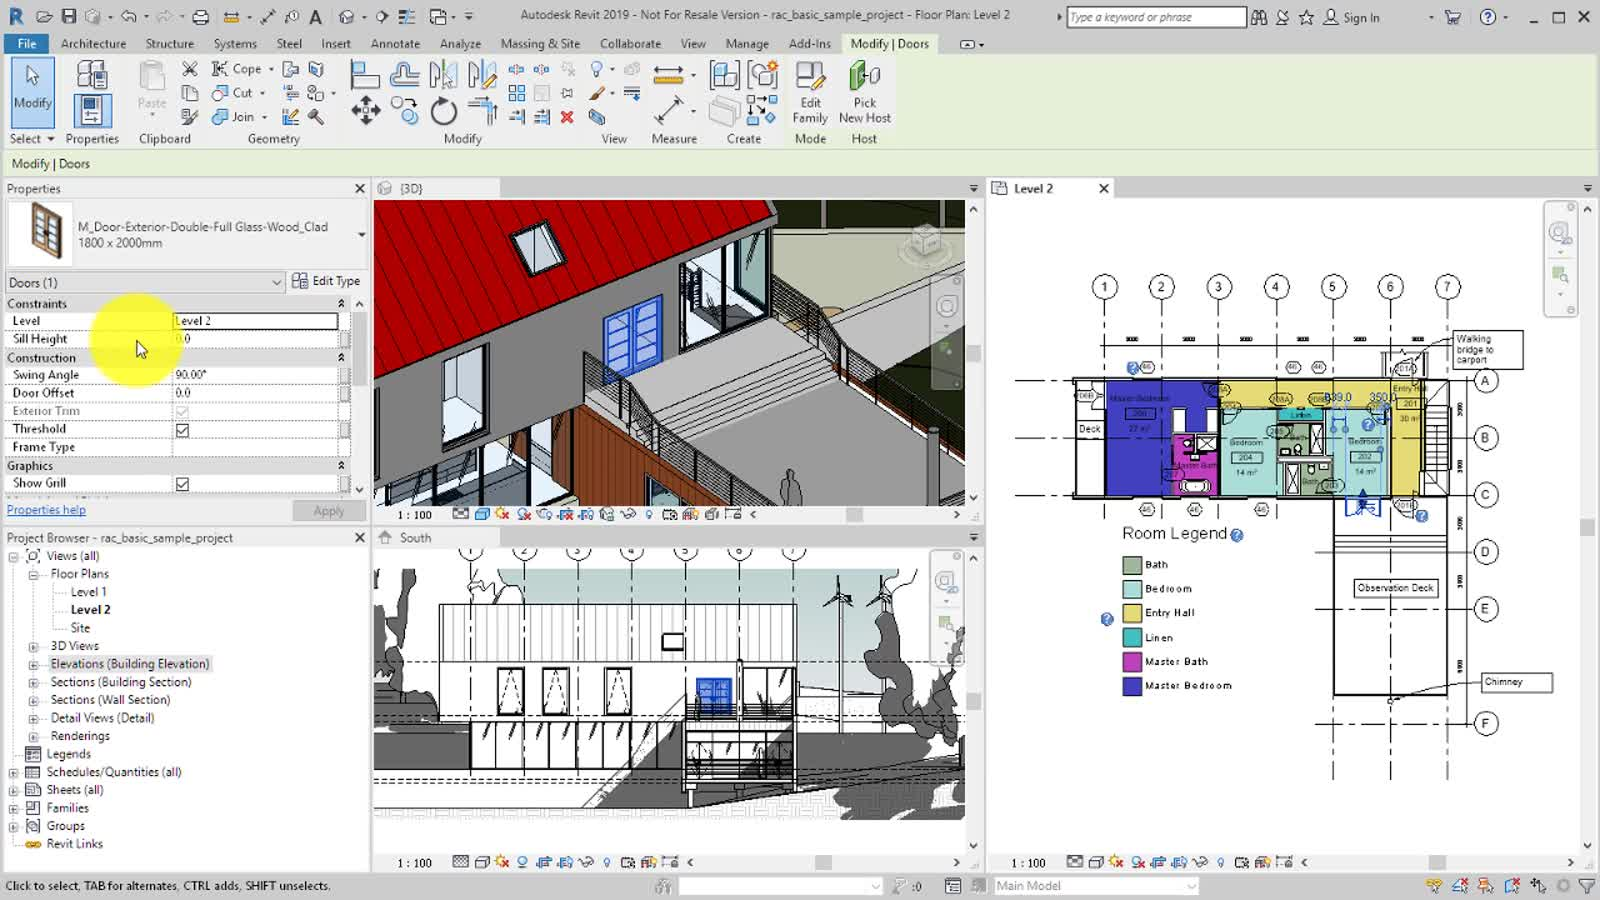
\includegraphics[width=0.9\textwidth, frame]{images/Revit-interface.jpg}
    \caption{Интерфейс редактора Revit.%
    \cite{DocRevit}}
    \label{figure:RevitInterface}
\end{figure}

Для хранения данных Revit использует специальный проприетарные форматы RVT, RFA и RTE.
Для отображения данных модели в виртуальной среде необходимо
преобразовывать их в форматы трехмерной графики, например OBJ или FBX.

\paragraph{Элементы информационной модели}

Каждая сущность в проекте информационной модели называется элементом.
Revit использует 3 типа элементов в проектах:
элементы модели, опорные элементы и элементы, относящиеся к представлению.
Элементы в Revit также часто называются семействами.
Семейство содержит геометрическое определение элемента и
параметры, используемые элементом.
Каждый экземпляр элемента определяется и контролируется семейством.%
\cite{DocRevit}
Для создания визуализации нас в первую очередь интересуют
именно элементы модели.

\begin{figure}[ht]
    \centering
    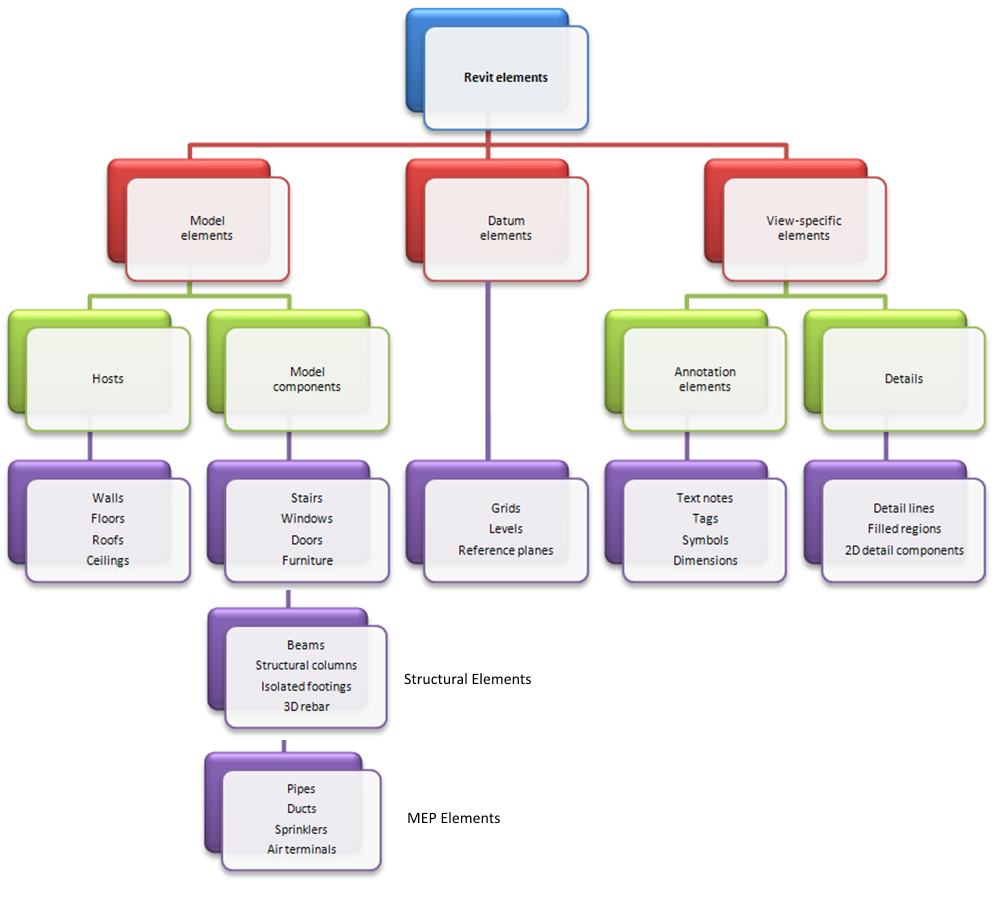
\includegraphics[width=0.9\textwidth]{images/Revit-elements.png}
    \caption{Элементы информационной модели.%
    \cite{DocRevit}}
    \label{figure:RevitElements}
\end{figure}

\begin{itemize}
    \item {
        Элементы модели.

        Элементы модели представляют фактическую трехмерную геометрию здания,
        например стены, окна, двери, пандусы,
        воздуховоды и электрические панели.
        Элементы модели делятся на хосты и компоненты модели.
        Хостами обычно являются элементы,
        которые возводятся непосредственно на строительной площадке,
        например стены и потолки.
        Компонентами модели являются все остальные типы элементов модели.
    }
    \item {
        Опорные элементы.

        Опорные элементы помогают определить контекст проекта.
        К ним относятся опорные плоскости, уровни и сетки.
    }
    \item {
        Элементы представления.

        Элементы представления это элементы,
        отображаемые только в каком-то определенном режиме представления проекта.
        Они помогают описывать или документировать модель.
    }
\end{itemize}

\paragraph{Свойства элементов}

Каждый размещаемый элемент является экземпляром семейства.
Элементы имеют 2 набора свойств, управляющих их внешним видом и поведением:
свойства типа и свойства экземпляра.%
\cite{DocRevit}

\begin{itemize}
    \item {
        Свойства типа.

        Один и тот же набор свойств типа является общим для всех элементов семейства,
        и каждое свойство имеет одинаковое значение для всех экземпляров определенного типа семейства.
        Изменение значения свойства типа влияет на все текущие и будущие экземпляры этого семейства.
    }
    \item {
        Свойства экземпляра.

        Общий набор свойств экземпляра также применяется ко всем элементам,
        принадлежащим к определенному типу семейства,
        но значения этих свойств могут различаться.
        Например, размеры окна являются свойствами типа,
        а его высота расположения над уровнем пола является свойством экземпляра.
    }
\end{itemize}


\subsection{Описание структуры клиентской и серверной части}
\label{subsections:ClientServerDesign}

Теперь можно поподробнее рассмотреть архитектуру прототипа.
Как было сказано ранее, основное предназначение приложения~--~
презентация информационной модели участникам проекта,
не имеющим навыков моделирования,
например заказчикам, спонсорам или непосредственным пользователям здания.
Такая презентация поможет успешнее вносить
корректировки в проект еще на самых ранних стадиях,
что снизит финальные затраты на реализацию проекта.%
\cite{Davidson2019}

Исходя из описанных требований можно сделать вывод о том,
что конечные пользователи приложения не станут использовать
программное обеспечение информационного моделирования.
Для них имеют значение только финальные или промежуточные результаты работы.
Поэтому было принято решение отделить функциональность приложения,
взаимодействующую с исходными данными модели.
Клиентская часть может не зависеть
от конкретной системы информационного моделирования,
что упростит расширение системы в дальнейшем.
Так же это может повысить производительность визуализации в клиентской части,
так как все трудоемкие вычисления, проводимые над исходными данными,
можно проводить на серверной части.

\paragraph{Функциональность серверной части}

Далее представлена основная функциональность реализуемая прототипом на "сервере".

\begin{itemize}
    \item {
        Хранение исходной информационной модели.
        
        Сервер должен хранить исходную модель,
        а также распознавать ее изменения для повторного преобразования.
    }
    \item {
        Конвертация формата RVT в формат FBX.

        Поскольку формат данных информационной модели отличается от
        представления классических форматов трехмерной графики
        и не поддерживается большинством фреймворков
        создания интерактивных графических приложений
        вроде Unity и Unreal, необходимо производить
        преобразование формата.
    } 
    \item {
        Предоптимизация модели.

        Из-за комплексности трехмерных моделей,
        получаемых после конвертации,
        необходимо проводить их дополнительную оптимизацию.
        Подробнее это будет рассмотрено в разделе~\ref{subsections:Optimization}.
    }
    \item {
        Упаковка моделей.

        Оптимизированные модели должны упаковываться для
        загрузки в клиентской части приложения.
    }
\end{itemize}

\paragraph{Функциональность клиентской части}

Далее описана функциональность клиентской части приложения
вместе с необходимыми схемами.
Функциональность, реализуемая не автором отчета,
а другими членами команды разработки, была опущена.

\begin{itemize}
    \item {
        Загрузка готовой модели.
        Приложение должно загружать выбранную упакованную модель.
        Так как в рамках прототипа не производится реализация удаленного сервера,
        загрузка будет происходить локально, как показано на рисунке~%
        \ref{figure:CModelLoader}.

        \begin{figure}[ht]
            \centering
            \includegraphics[width=0.6\textwidth]{example-image}
            \caption{Загрузчик моделей.}
            \label{figure:CModelLoader}
        \end{figure}

        \intextcomment{
            Описание UML-схемы...
        }
    } 
    \item {
        Размещение модели в виртуальной среде.
        После загрузки модель должна размещаться в виртуальной сцене.
        Для визуализации будет использоваться виртуальный стол,
        на который будет проецироваться модель здания
        в уменьшенном масштабе согласно схеме на рисунке~%
        \ref{figure:CStand}.

        \begin{figure}[ht]
            \centering
            \includegraphics[width=0.6\textwidth]{example-image}
            \caption{Размещение модели.}
            \label{figure:CStand}
        \end{figure}

        \intextcomment{
            Описание UML-схемы...
        }
    } 
    \item {
        Взаимодействие с элементами модели.
        После размещения модель будет разбивать на слои,
        представляющие отдельные структурные элементы здания,
        например стены, лестницы или двери.
        На каждый отдельный слой может накладываться эффект,
        изменяющий его отображение.
        На рисунке~\ref{figure:CLayers} показана
        структура системы слоев.

        \begin{figure}[ht]
            \centering
            \includegraphics[width=0.6\textwidth]{example-image}
            \caption{Система слоев.}
            \label{figure:CLayers}
        \end{figure}

        \intextcomment{
            Описание UML-схемы...
        }
    } 
\end{itemize}

\comment{
    TODO:

    Запилить UML!
}



\subsection{Обзор оптимизационных подходов}
\label{subsections:Optimization}

Теперь можно рассмотреть подходы повышения производительности визуализации.
Важность этого аспекта была выявлена 
ещё на самых ранних стадиях разработки прототипа.
Информационные модели зачастую обладают очень комплексной геометрией.
Более того, визуализация в виртуальной реальности накладывает
дополнительные ограничения, так как изображение проходит двукратную отрисовку
из-за наличия двух глаз с разной перспективой.
В добавок к этому низкая частота кадров в виртуальной реальности
может вызывать плохое самочувствие у пользователя.%
\cite{Weech2019}

\paragraph{Вспомогательные понятия}

\begin{rglossary}
    Для начала введем несколько вспомогательных терминов:

    \rglossarylineExpl{Draw call}
    {рус. Вызов отрисовки}
    {команда отрисовки полигональной сетки,
    отдаваемая центральным процессором графическому.}

    \rglossarylineExpl{Шейдер}
    {англ. shader}
    {разновидность компьютерных программ, запускаемых на графических процессорах,
    предназначенных для отрисовки изображений.}

    \rglossarylineExpl{Меш или полигональная сетка}
    {англ. polygon mesh}
    {структура данных, содержащая набор вершин, ребер и граней,
    определяющих форму многогранного объекта.}

    \rglossaryline{Графический материал}
    {набор данных, ассоциируемый с моделью и
    определяющий то, как будет отрисована ее поверхность
    в зависимости от выбранного шейдера.}
\end{rglossary}

\paragraph{Распространенные причины проблем с производительностью}

\begin{itemize}
    \item {
        Сложная геометрия модели. Под сложной геометрией понимается
        большое количество полигонов (граней) в полигональной сетке модели.
    }
    \item {
        Большое количество draw call'ов.
        Выполнение запроса на отрисовку выполняется центральным процессором и
        является достаточно трудоемкой операцией. За один вызов может быть
        обработана только одна полигональная сетка.
        Вполне возможна ситуация, при которой центральный процессор тратит больше времени,
        чтобы инициировать отрисовку, чем графический процессор будет ее исполнять.
    }
    \item {
        Трудоемкие шейдеры. Алгоритм шейдера может иметь
        высокую вычислительную сложность
        (например использовать долговычислимые тригонометрические функции) или
        иметь неподходящую структуру для запуска на графическом процессоре
        (например содержать многочисленные ветвления).
        Помимо этого работа шейдера может предполагать неоднократную
        отрисовку объекта для достижения определенного результата.
    }
\end{itemize}

\paragraph{Существующие подходы}

\begin{itemize}
    \item {
        Visibility culling (Отбор видимых полигонов).

        Visibility culling~--~это семейство алгоритмов,
        нацеленное на предотвращение вызовов отрисовки
        для объектов невидимых в кадре.%
        \cite{Cohenor2002}
        Пример различных техник отбора видимых полигонов
        показан на рисунке~\ref{figure:CullingTechniques}.
        Подобные алгоритмы являются очень эффективными,
        когда количество объектов единовременно видимых в виртуальной сцене
        значительно меньше их общего количества,
        например в замкнутых помещениях внутри крупного здания.

        \begin{figure}[ht]
            \centering
            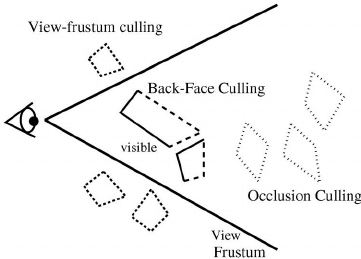
\includegraphics[width=0.8\textwidth]
            {images/Three-types-of-visibility-culling-techniques.png}
            \caption{Техники отбора видимых полигонов.%
            \cite{Cohenor2002}}
            \label{figure:CullingTechniques}
        \end{figure}

        \begin{itemize}
            \item {
                View-frustum culling~--~это техника отбора,
                отсекающая отрисовку объектов,
                находящихся за границами поля зрения виртуальной камеры.
            }
            \item {
                Back-face culling~--~это техника отбора,
                позволяющая избежать отрисовку геометрии,
                направленной в противоположную сторону от виртуальной камеры.
            }
            \item {
                Occlusion culling~--~это техника отбора,
                предотвращающая отрисовку геометрии,
                скрытой за другими объектами виртуальной сцены.
            }
        \end{itemize}
    }
    \item {
        LOD (англ. Level of detail~--~уровень детализации).

        LOD~--~это оптимизационная техника,
        нацеленная на снижение используемого количества
        полигонов модели при ее удалении от виртуальной камеры.
        Для работы метода требуется создать несколько версий
        одной и той же модели с разным уровнем детализации (количеством полигонов),
        как это показано на рисунке~\ref{figure:LOD0-1}.

        \begin{figure}[ht]
            \centering
            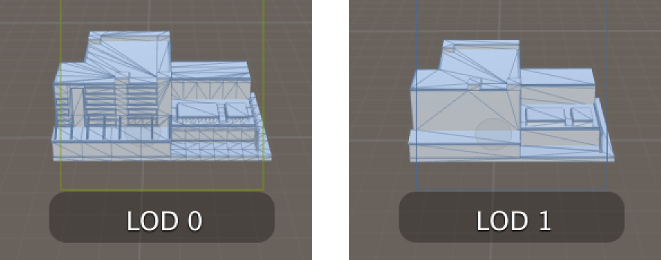
\includegraphics[width=0.8\textwidth]{images/LOD0-1.png}
            \caption{Разные уровни детализации.%
            \cite{DocUnity}}
            \label{figure:LOD0-1}
        \end{figure}

        Перед вызовом запроса отрисовки производится выбор необходимой модели,
        то есть вблизи от виртуальной камеры будут отрисовываться
        детализированные модели (LOD0), а вдали упрощенные (LOD1-LOD3).
    }
    \item {
        Batching.

        Батчинг~--~это оптимизационная техника,
        предназначенная для снижения количества запросов отрисовки
        за счет группировки нескольких полигональных сеток.

        \begin{itemize}
            \item {
                Батчинг может происходить динамически, если
                группируется множество простых объектов,
                с одинаковыми графическими материалами и текстурами
                (чего можно добиться с помощью создания атласа текстур).
                За счет этого можно отрисовывать несколько движущихся объектов
                за один вызов отрисовки, что имеет смысл, если продолжительность
                группировки меньше, чем затраты на многочисленные вызовы отрисовки.
            }
            \item {
                С другой стороны батчинг может быть статическим, то есть
                происходить однократно и объединять неизменяемую геометрию
                в одну полигональную сетку, позволяя достичь ещё большей производительности,
                чем при динамической группировке.
                Стоит отметить, что подобная группировка снижается
                эффективность отбора видимых полигонов, так как
                сгруппированные объекты начнут восприниматься как один.
            }
        \end{itemize}
    }
    \item {
        Geometry instancing (Дублирование геометрии).

        Geometry instancing~--~это методика, позволяющая
        одновременно рендерить нес\-колько объектов, имеющих
        одинаковую полигональную сетку.
        Такой подход в основном используется для отрисовки
        повторяющихся фоновых объектов, таких как растительность или здания.
        Объекты могут иметь разное положение в пространстве,
        размеры, отличающиеся графические материалы.
        Дублирование геометрии значительно снижает
        количество запросов на отрисовку.
    }
\end{itemize}

\paragraph{Выбранный подход}

При разработке прототипа было принято решение
использовать вариацию статического батчинга,
при котором полигональные сетки всех объектов одного слоя
(описано ранее в разделах~\ref{subsections:DomainModel}
и \ref{subsections:ClientServerDesign})
объединяются в одну на одном из этапов конвертации
исходной информационной модели.
В дальнейшем этот подход может быть пересмотрен,
так как несмотря на продемонстрированную эффективность
он обладает рядом недостатков,
а именно пропадает возможность взаимодействия с
отдельными объектами слоя, а также
теряется значительная часть атрибутивной информации.
